\begin{pastexam}[label={px:ncu-114-dsa-04}]{中央資工所 114 學年度 第 4 題}
（複選；每題 5 分，全部答對才給分，答錯倒扣 1 分）

A binary tree has inorder traversal, \textbf{ILOVENCU}, and postorder traversal, \textbf{ILVNCUEO}.
Which of the following statements is (are) true?
\begin{enumerate}[label=(\alph*)]
\item The fifth letter in the level-order traversal is V
\item The height of the binary tree is 4
\item C is a leaf node
\item The sixth letter in the level-order traversal is U
\end{enumerate}
\end{pastexam}

\begin{pastsoln}
答案：(a)(b)(d)。

(b) 和高度的定義有關。 題目是英文卷，高度採英文教科書（CLRS）的定義：根到最深葉節點的\textbf{邊數}。
資結書第~7.1~節數的是節點數（層數），用那個定義這棵樹的高度是 $5$，(b) 就變成錯的。

\textbf{重建}（資結書第~7.4~節）。 後序的最後一個是根，在中序裡找到它，左邊是左子樹、右邊是右子樹；
後序裡左子樹的部分在前、右子樹的部分接在後面，長度和中序的兩段一樣。
\begin{itemize}
\item 後序最後是 O。 中序 \texttt{IL\,|\,O\,|\,VENCU}：左子樹中序 IL、右子樹中序 VENCU。 後序的前
$2$ 個 IL 是左子樹，接著 VNCUE 是右子樹。
\item 左子樹：中序 IL、後序 IL。 根 L，I 在 L 的左邊，是 L 的左子。
\item 右子樹：中序 VENCU、後序 VNCUE。 根 E；中序 \texttt{V\,|\,E\,|\,NCU}，左子 V，右子樹中序 NCU、
後序 NCU。
\item 中序 NCU、後序 NCU：根 U；中序 \texttt{NC\,|\,U}，只有左子樹，中序 NC、後序 NC。
\item 中序 NC、後序 NC：根 C，N 在 C 左邊，是 C 的左子。
\end{itemize}
\begin{center}
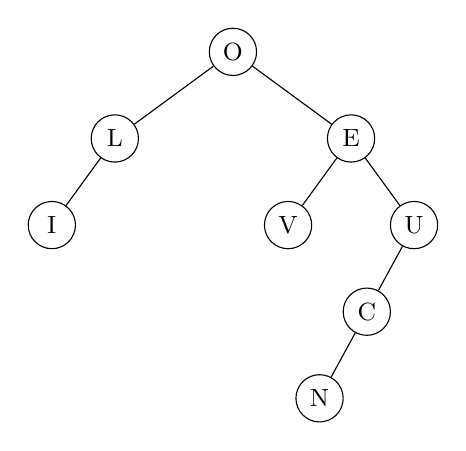
\begin{tikzpicture}[level distance=11mm,
  every node/.style={circle,draw,inner sep=1pt,minimum size=6mm,font=\small},
  level 1/.style={sibling distance=30mm}, level 2/.style={sibling distance=16mm},
  level 3/.style={sibling distance=12mm}]
\node {O}
  child {node {L} child {node {I}} child[missing]}
  child {node {E}
    child {node {V}}
    child {node {U}
      child {node {C} child {node {N}} child[missing]}
      child[missing]}};
\end{tikzpicture}
\end{center}
檢查：這棵樹的中序是 I L O V E N C U，後序是 I L V N C U E O，和題目一樣。

\textbf{層序}（資結書第~7.3.2~節）。 第 $1$ 層 O；第 $2$ 層 L, E；第 $3$ 層 I, V, U；第 $4$ 層 C；
第 $5$ 層 N。 層序是 \texttt{O L E I V U C N}。

逐項檢查：
\begin{itemize}
\item (a) 第 $5$ 個是 V。 對。
\item (b) 最深的 N 在第 $5$ 層，根到 N 的路徑 O--E--U--C--N 有 $4$ 條邊，高度 $4$。 對（見第一段）。
\item (c) C 有左子 N，不是葉節點。 錯。
\item (d) 第 $6$ 個是 U。 對。
\end{itemize}
\end{pastsoln}
